\documentclass[iop,apj]{emulateapj}
\usepackage{amsmath, amssymb, amstext}
\usepackage{todonotes}
\usepackage[breaklinks, colorlinks, citecolor=blue, linkcolor=magenta]{hyperref} 
\renewcommand*{\sectionautorefname}{Section}
\usepackage[all]{hypcap}
\usepackage{aas_macros}
\usepackage{natbib}
%\linespread{2.5}
\bibliographystyle{apj}
\shorttitle{Short Title}
\shortauthors{Author et al.}
\begin{document}

\title{Detecting Active Asteroids/Comets from OSSOS survey images}
\author{Authors}
\affil{Affiliations}

\begin{abstract}
Abstract.
\end{abstract}

\keywords{keywords}
\maketitle

\section{Introduction}

Until the last few decades, comets and asteroids have been thought of as separate populations differing in  both morphology and dynamics. With different fractions of volatile content, an obvious distinction is the presence of a transient coma and/or tail around a comet, whereas asteroids exhibit bare nuclei photometric properties. [todo: mention Tisserand parameter here?]  With the recent advent of large wide-field surveys which have regularly monitored large populations of solar system bodies, objects which exist between the classification of comets and asteroids have been discovered. The classical view of comets being rocky ice bodies with highly eccentric orbits, and asteroids being icy rock bodies with stable orbits confined to the main asteroid belt between Mars and Jupiter \citep{sheppard15}, has been supplanted by the discovery of comet-asteroid transition objects. Asteroids in comet-like orbits, dynamically asteroidal objects that exhibit burst of cometary activity or are associated with meteor streams such as the Damocloids (\cite{sonnett11}; and references therein, \cite{gilbert09}) exist between the accustomed classification criteria. These objects may be comets which have exhausted their volatile content or are dormant, or asteroids which have a higher volatile fraction. In this study we focus on the ``Active Asteroids'' (AAs) (or main belt comets (MBCs)) \citep{hsieh06}, which are a population of bodies with stable asteroid-like main belt orbits that exhibit transient mass loss forming comae and/or tails consistent with cometary morphology.  

As it is expected that icy objects in the inner solar system would have long ago sublimated, the active asteroids pose an interesting insight to the heliocentric distance at which ice condenses, known as the `snow line', which of interest to planetary formation and determining the chemistry of the early solar nebula. For objects which formed in the the outer region of the main belt, the crystallized water ice which was present at the time of formation and not exposed to primordial heating may still remain in reservoirs beneath the surface \citep{prialnik09}.  According to models developed by \citet*{fanale89},  beyond heliocentric distances of 2.4 AU ice can be protected against sublimation by a relatively thin surface regolith  of depth 1 -- 100 m for the entire age of the solar system. If the ice layer were to be exposed to sub solar heating by an impact or other triggering event, sublimation could eject dust particles from the surface. The source of the dust emission may be different for each object and could include ice sublimation, impact ejecta, rotational instabilities due to YORP torques, or a combination of several effects (\cite{jewitt15}; and references therein).  

%The active asteroids are small bodies in the main asteroid belt which have transient dust emission producing comet-like comae and tails. Unlike comets, which originate in the Kuiper Belt and Oort cloud, and have been scattered inwards by gravitational effects, the active asteroids have stable orbits confined to the main belt and likely formed in the same location as they reside presently \citep{sheppard14} \citep{fernandez02}. 
% A standard criterion for interpreting the differing dynamics between the comet and asteroid populations is the Tisserand parameter, with respect to Jupiter, where comets have a value less than three, and asteroids greater than three.  It has been observed that asteroids may have comet-like orbits \citep{gilbert09} (and references within) and there are also objects with cometary properties in asteroid-like orbits (active asteroids or main belt comets). Since the discovery of these intermediate type objects, the classification criteria for asteroids and comets has become less obvious.

% impacts inferred from observed large brightening and quick fading 
% sublimation inferred from prolonged or periodic activity during perihelion passage, Hsieh et al 2010, 2011
%The ejected dust would form a coma around the object, and radiation pressure affects would then (preferentially) push the smaller particles away from the asteroid forming a tail.
%Sublimation driven active asteroids differ from comets in that the comets, having larger ice reservoirs, would have stronger sublimation events which could eject larger debris. The cometary tail would then be longer lived as the larger debris would be less affected by the radiation pressure, and thus dissipate slowly. It is also possible, however, that prolonged activity is a result of ongoing ejection of small, fast dissipating particles. \cite{TEST} 

Since the first discovery of an active main-belt asteroid, 133P/Elst-Pizarro \citep{elst96}, several attempts have been made to identify new objects of this type; at present, nineteen objects have been identified with diverse set of orbital dynamics, see Figure 1 \citep{jewitt15, hsieh15}. A comprehensive review of these surveys can be found in \citet{hsieh15}.  A persistent challenge to this effort is that the detection of the faint coma or tails around small dark objects is highly dependent on the magnitude constraints of the survey. As most asteroids fall near the limiting magnitude of the survey in which they are discovered \citep{jewitt15}, objects which are larger, closer, or have higher albedo are preferentially detected and any dust emission would be more easily apparent. At present, the active fraction of identified active asteroids greater than 1 km to main belt asteroids greater than 1 km is approximated as $f \, \sim \, 10^5$, and describes a strong lower limit as many objects are yet undetected. \citep{jewitt15} %From a study of 30,000 objects observed near perihelion, \cite{} Hsieh et all (2015) concluded that $f \, \sim \, 10^4$ for asteroids which are active at any instant in the outer belt.

\begin{figure}[!htb]
    \centering
    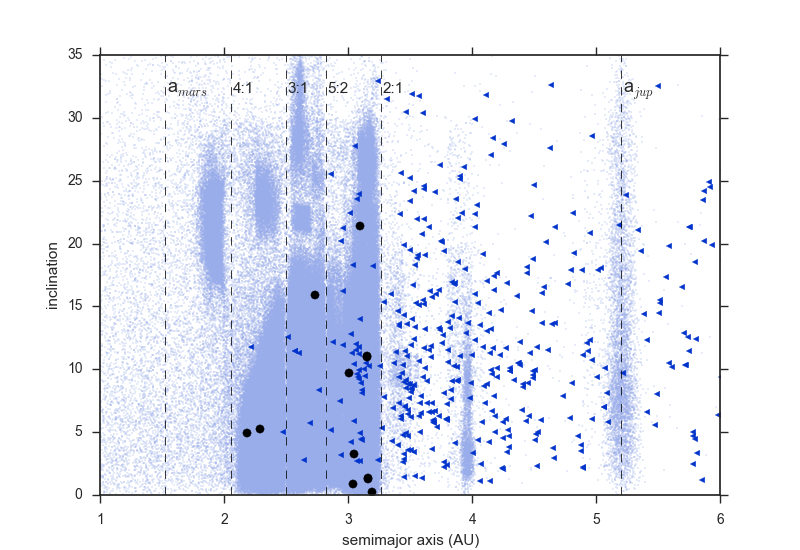
\includegraphics[width=\linewidth]{graphs/aa_comets_mba_all.png}
    \caption{Inclination of all objects in the main asteroid belt from the AstDys catalogue as a function of semimajor axis.  Mean motion resonances between Mars and Jupiter as well as the planet's semimajor axis are marked in dashed lines, main belt objects are marked as light small dots, comets as arrows, and active asteroids as stars.}\label{fig:1}
\end{figure}

In this paper, we present a study of main belt objects present in the Canada-France-Hawaii Telescope (CFHT) Outer Solar System Origins Survey (OSSOS) data to search for evidence of cometary-like activity in asteroidal bodies. Previously undetectable emission activity may be able to be identified in the OSSOS survey, which has a limiting magnitude much lower than previous surveys. Potential activity is identified by measuring the asteroids brightness profile and comparing this to a stellar model profile of the same magnitude in order to detect a large deviation in width potentially characteristic of a coma or jet. Asteroids which have residuals larger than a 3 sigma deviation are subjected to visual examination. This is similar to the process employed by \cite{luu92}, \cite{sonnett11}, and \cite{gilbert09}.

We select three test groups to ensure the efficiency of our search. The first is the Hungaria family, which is a population of bodies in the inner edge of the main asteroid belt at relatively high inclination and low to moderate eccentricity \citep{milani10}. This family was chosen as it's relative closeness means that the majority of the population should be visible within the limiting magnitude, and that it is thought to be a very dynamically active population. Surrounding the Hungarias are dynamically unstable boundaries with a strong perihelion resonance with Jupiter, the node of the orbit locked to the node of Saturn, and an interaction with the orbit of Mars. As the region is populated by bodies through to be native to the region, and as a result of collisional interactions of large parent bodies \citep{milani10}, it is possible that ongoing collisions could still reveal submerged volatile content. However, due to the low semi-major axis, it is likely that any exposed water ice would dissipate quickly. 
Three known active asteroids are present in the current OSSOS data, however their current activity is unknown. We also include images of a unreported comet during its period of activity discovered in the CFEPS survey to ensure that our pipeline can accurately identify a coma with reasonable certainty.


\section{Observations}

Observations taken by OSSOS with the CFHT MegaPrime wide-field optical imaging facility at the summit of Mauna Kea, Hawaii, have been collected since February 2013. The wide-field imager MegaCam is a 36 CCD image plane, each 2048 x 4125 CCD with resolution of 0.185"/pix. This covers a field of  $\sim$ 1$^{\circ}$ x 1$^{\circ}$ on the sky. Each block of data taken consists of a mosaic of 21 segments of one-square-degree sky coverage, and at present, covers two orbital phase spaces on the plane of the ecliptic, and two off plane at low inclinations. The OSSOS survey employs the u* and r' filters on the MegaCam with integration times of 287, 387, and 500 seconds, yielding a lower limit of $m_r \, \sim$ 24.5 magnitudes.

The OSSOS images were pre-processed by standard data detrending with the MegaPipe image stacking pipeline [todo: check if this is correct]. An astrometric correction was applied by [todo: sgwyn, check if there is a reference]. Source characteristic measurements were obtained from Source Extraction and Photometry in Python (SEP) and were used to extract the orbital information the transient objects. 

The survey covers a wide field of both the ecliptic plane and low inclinations allowing for the observation of a large number of main belt objects in different orbital phase spaces. This can be seen in Figure 2. As the observations were not targeted to specific main-belt populations, the survey is relatively unbiased, and we can improve the constraints on the number of AAs  in the whole of the main asteroid belt. 

\begin{figure}[!htb]
    \centering
    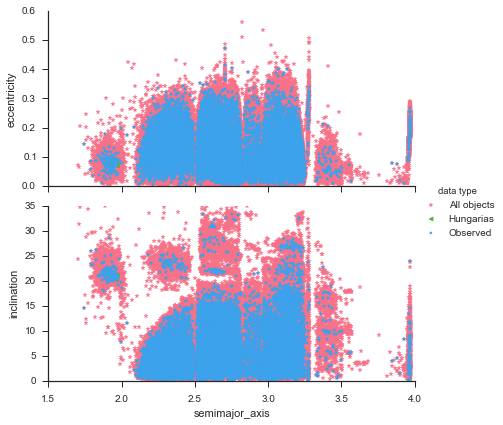
\includegraphics[width=\linewidth]{graphs/obs_e_i.png}
    \caption{Objects observed in the OSSOS data set overlaid on all of the known objects in the asteroid belt for inclination and eccentricity as a function of semi-major axis.}\label{fig:2}
\end{figure}

\begin{figure}[!htb]
    \centering
    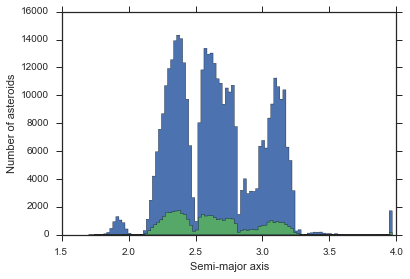
\includegraphics[width=\linewidth]{graphs/hist_a.png}
    \caption{The number of asteroids and number of asteroids observed as a function of semi-major axis.}\label{fig:3}
\end{figure}

\section{Analysis}

From the calculated arcs provided by the Solar System Object Image Search (SSOIS) ephemeris \citep{ssois} of 671,234 main belt objects in the Asteroids Dynamic Site (AstDys) catalogue \citep{astdys} we were able to predict which asteroids were present in the OSSOS data set and could be examined for cometary activity. From a set of 3,528 images, there are 201,477 observations in the \textit{r} band of 46,367 objects in the OSSOS data. We analyze a small group of objects in the Hungaria family as our test case for our automated pipeline. Of the 1187 Hungarias we have 76 observations of 25 objects, of the known AAs we have 11 observations; 3 of 238P/Read, 6 of P/2012 F5 (Gibbs), and 2 of (2201) Oljato.  A detailed discussion of each of these AAs can be found in \cite{jewitt15}. And we have 5 observations of an unreported active comet from the CFEPS data set.

We use a two-step pipeline to locate the asteroid in the image, and then measure the brightness profile of the point spread function (PSF). The profiles are then compared to stellar models, with significant deviations between the profiles indicating potential activity.

\begin{figure}[!htb]
    \centering
    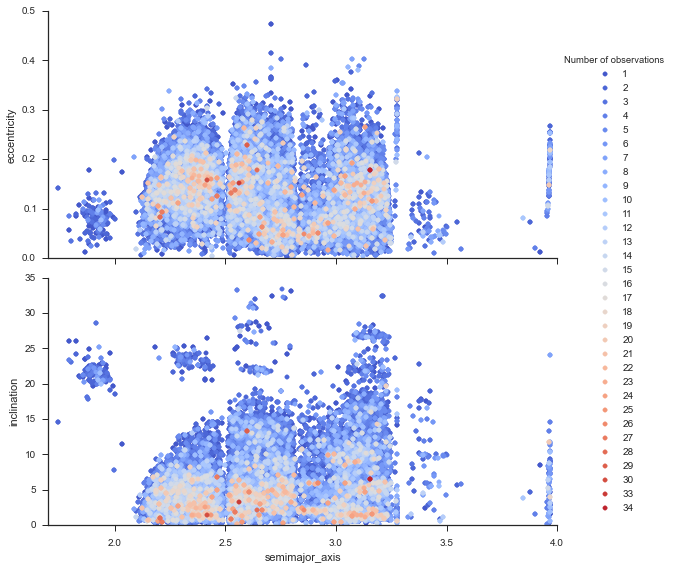
\includegraphics[width=\linewidth]{graphs/occurance2.png}
    \caption{The number of observations of asteroids in the OSSOS data set organized by inclination and eccentricity as a function of semi-major axis.}\label{fig:4}
\end{figure}

\begin{figure}[!htb]
    \centering
    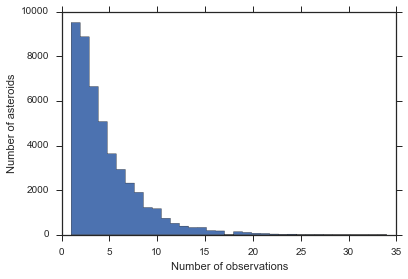
\includegraphics[width=\linewidth]{graphs/hist_obs.png}
    \caption{The number of observations by OSSOS of each asteroid.}\label{fig:5}
\end{figure}

[absolute magnitude graph??]

\subsection{Object identification}

An automated pipeline was written to identify each asteroid in an OSSOS exposure by: location relative to the predicted coordinates,  elongation due to trailing effects caused by the apparent rate of motion over the duration of the exposure, and apparent magnitude. 

The coordinates of each object in the exposure were obtained from the photometric software SEP, and objects which were closest to the predicted location (at the midpoint of the exposure) as calculated by known arc \citep{jpl} [todo: is this citation necessary?] were chosen as candidate objects. If no objects were detected within a set radius calculated from the uncertainty in the asteroid arc, the radius was increased by a factor of 1.5 and the search was repeated.

The predicted elongation of the trail was calculated from the motion of the asteroid over the length of the exposure \citep{jpl} under the assumption of constant motion. This was compared to the elliptical shape parameters measured by SEP for each candidate object. 
A difficulty in this process is that objects which move faster during the exposure, and thus have longer trails, will be less elliptical in shape. As the photometry software is optimized for point sources and extended sources such as galaxies, the accuracy of the shape parameters to be correlated to the extent of the elongation. For this reason we implement an uncertainty of 20 percent on the elongation measure, with the expectation that only objects which are markably inconsistent would be rejected. For greatly extended trails, with a ratio of semi-major axis to semi-minor axis of 5:1, SEP incorrectly resolves the asteroid as two separate objects as the flux spread was not necessarily constant over the length, see Figure 6. In this case both objects would meet the location and magnitude conditions, pass through the same consistency level, and be flagged for visual inspection. The accuracy of this process could be significantly improved with the inclusion of a trail fitting algorithm in the photometry software.

\begin{figure}[!htb]
    \centering
    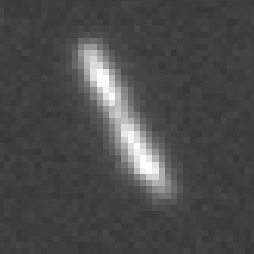
\includegraphics[width=0.4\linewidth]{images/flux_spread.png}
    \caption{A Fast moving asteroid trailed over the duration of the exposure with an uneven flux spread over its length. This object required visual inspection as  it was incorrectly resolved as multiple objects by SEP}\label{fig:6}
\end{figure}


The inability of the photometry software to correctly measure the shape of the asteroid trail would also affect the accuracy of the flux measurement as the aperture may not include the total amount of light. As the centre of the object is determined by the flux weighted barycenter of the object, this may also result in an inaccurate measurement of the astrometry. In order to avoid this error, the centre coordinates of the object were chosen as the centre of the elliptical aperture for fast-moving objects. 
In addition, the elongation effect in itself may affect the accuracy of the flux measurement without taking into account the potential loss of light. This is a result of the flux being spread over a larger area than the point spread function (PSF), which reduces the per unit area apparent magnitude and the signal-to-noise \citep{veres12}. A direct consequence is a lowered limiting magnitude for fast moving asteroids. 
A third consideration is that objects which are active and have jets or a coma will appear brighter than the expected magnitude calculated from previous observations. Depending on the extent of the activity, this could cause the object to be measured as several magnitudes greater than predicted. For these reasons, in subjecting the candidate object to a consistency check with the predicted value we used an uncertainty of 2 magnitudes (unless the object was predicted to vary by a larger amount in the span of 10 days following the exposure) and did not reject the object if it was inconsistent.

In order to accurately measure the PSF of the asteroid it is necessary to ensure that the asteroid is isolated from other sources. A catalogue of bright sources [todo: cite gwyn?] was built for the OSSOS data set from a collection of exposures with excellent photometry, and was used to ensure that the asteroids were not involved with a background source.

%In order to reject asteroids which were involved with background objects, the coordinates of the object were compared to a catalogue of bright sources built for the OSSOS data set. This will not, however, detect if the asteroid is involved with a faint background source nor a transient object such as a cosmic ray. It is possible that the involvement would cause the object to be rejected based on the measured elongation or shape. 

A candidate object which did not meet any of the criteria mentioned above would be examined visually. Objects which met the location and elongation conditions were preferentially selected over those that only met the location and magnitude conditions. If multiple objects met the same level of criteria, they would also be examined visually.

%This would include objects which were involved with or too close to bad pixels or cosmic rays, on the edge of the CCD, in a diffraction ring of a nearby bright star (but far enough spatially to not be rejected as involved), or that could not be accurately measured by the photometry software.

Applying this identification process left 66 exposures of 21 asteroids to be examined.

\begin{table}[htdp]
\caption{Rejection cause for images through identification pipeline}
\begin{center}
\begin{tabular}{lc}
	Total number of images							&	76 			\\
	\hline
	\textbf{Rejection cause}						& 	\textbf{\# images} \\
	\hline
	Involved with background stars                          & 	1			\\
	% 129991 1795922p
	Off the edge of the CCD						& 	5			\\
	% 111753 1774672p
	% 204248	1672758p
	% 204248	1672759p
	% 204248	1672780p
	% 204248	1672810p
	In saturated region of nearby bright star			& 	1			\\
	% 159176 1667550p
	In diffraction region of nearby bright star		&	1			\\
	% 283374	1769004p
	% 283374 1775265p
	Bad exposure									& 	4			\\
	% 283374 1775274p
	% 204248 1672749p  # No data in this HDU.
	% 204248 1672750p  # No data in this HDU.
	% 204248 1672754p
	\hline
	Cause for visual inspection						&	\textbf{\# images} \\
	Incorrectly resolved as multiple objects			&	x1			\\
	Did not meet elongation condition				&	x2			\\
	Retained										&	64 - x1 - x2
\end{tabular}
\end{center}
\label{default}
\end{table}

\subsection{Rejection causes}

\textit{Involved}:
When compared with a catalogue of bright sources [todo: cite Gwyn?] the object was found to spatially coincide with a background object. As the catalogue was built from a set of exposures with good photometry, asteroids present in those exposures would be incorrectly identified as involved. [todo: can we get a list of the exposures used?] Not included in the catalogue are dim sources, transient objects, and bad pixels/columns. In the case of the asteroid being involved with such objects, the photometry software would measure the convolved sources, and the elongation and magnitude would be inconsistent with the predicted values. If the background object were dim enough that the convolved source passed the magnitude condition, the PSF would be beyond the 5 sigma deviation, and the involvement would be caught by visual inspection. An example of such a case is shown in Figure 2 [todo: reference figure].

\textit{Not on the CCD}:
If the SSOIS query incorrectly identified that an asteroid was on in an OSSOS exposure, but rather the object was within a few degrees off the edge of the CCD, no object would be found in the uncertainty ellipse of the predicted location.

\textit{In saturated region of a nearby bright source}:
For object close to, but not involved with, bright sources the asteroid may in the diffraction region of the saturated pixels. In this case no object would be found in the uncertainty ellipse around the predicted co-ordinates.

\textit{Bad exposure}:
Exposures which were marked as bad were automatically rejected. This would include tracking errors, short exposures, poor image quality, and corrupted images. 

\subsection{PSF profile comparison}

A postage stamp of size 2.5 times the full-width-half-maximum (FWHM) and centred on the midpoint of the elongated shape was rotated such that asteroid trail was aligned parallel to the pixel rows on the CCD chip. The asteroid profile was averaged over the entire length of the postage stamp. The stellar model PSF was built from the OSSOS MOP at the location of and with the same magnitude as the asteroid on the CCD to account for any distortion, and rotated by the same angle.  The profile was measured as the average over the width of the model star. 

Due to saturation effects, asteroids with magnitudes greater than 18.5 were not analyzed for activity by this process, but instead reviewed visually. As a stellar profile model has not, at the present time, been built for all the OSSOS data, but only for the latest data set, the older images were also reviewed visually. 

A 3 sigma difference between the subtracted profiles was used to indicate the presence of additional flux around an asteroid, characteristic of a cometary comae. Each asteroid with at least two points with greater than a 3 sigma deviation were retained for visual inspection.

The profiles of the asteroids were examined for asymmetric features (such as would result from a jet) and extended wings (such as would result from a coma) when compared visually to the stellar model profile. An asteroid profile not indicating activity and that of a comet is shown in Figure 4. 

\begin{table}[htdp]
\caption{Cause for visual inspection}
\begin{center}
\begin{tabular}{lc}
	Retained from identification process			&	66 			\\
	\hline
	\textbf{Visually inspected}						& 	\textbf{\# images} \\
	\hline
	Above 18.5 magnitude			                          & 	2			\\
	No stellar model								&	15			\\
	\hline
	Retained										&	49
\end{tabular}
\end{center}
\label{default}
\end{table}

\begin{figure}[!htb]
    \centering
    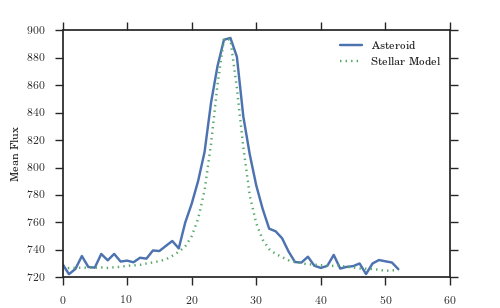
\includegraphics[width=\linewidth]{images/asteroid_psf_broad_10477.png}
    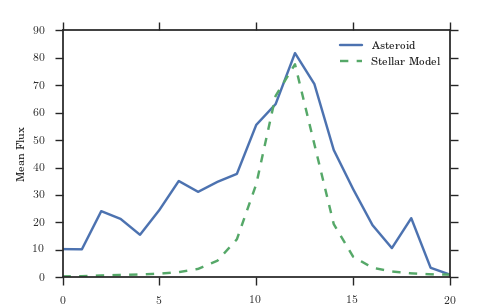
\includegraphics[width=\linewidth]{images/comet_psf3.png}
    \caption{Top: A brightness profile of an asteroid is shown as a blue solid line, and that of the stellar model is shown as a green dashed line. The asteroid profile shows little deviation from the stellar profile, indicating bare photometric properties, and that no activity is present. Bottom: A brightness profile of a comet is shown as a blue solid line, and that of the stellar model is shown as a green dashed line. [todo: comment on comparison]}
    \label{fig:4}
\end{figure}

\subsection{Known comet test }

Tests as of yet are inconclusive.
% No activity was detected on 238P/Read, P/2012 F5 (Gibbs), nor (2201) Oljato. The comet identified in the CFEPS images.




\subsection{Detections}

Of the 49 images where the brightness profile was measured, 3 asteroids were have a 3 sigma deviation from the stellar model profile. All of the asteroids were overlapping the CCD edge or saturated pixels making the object appear more extended.

How well do we identify coma vs jets vs tails ? How may do we detect vs observed? What are the statistics? Why are the results so bad?

\section{Discussion}

\subsection{Identification criteria}

The given uncertainty of 20 percent was found to be a robust [todo: WC?] as the percent difference between the predicted and measured elongations for all objects correctly measured by SEP was under 18 percent, and with a mean of 8 percent. This was therefore a good value for only rejecting objects which were not the intended asteroid or not properly measured.

Despite the expectation that the elongation would be correlated to the inaccurate measurement of the magnitude due to the spread of the flux, no statistical relationship was found between the difference of the predicted and measured magnitude and the elongation.

\subsection{Photometry errors}



All objects which were successfully identified passed the elongation condition
How many objects were `very' elongated?


As the involvement test was preformed from a catalogue of bright objects, it is possible that asteroids involved with dim background objects were not properly flagged. An example of this is shown in Figure 4. Depending on the geometry of the involvement this could be selected as an asteroid with activity, possibly with a large bright jet. The involvement would then be determined in the visual examination of all asteroids with brightness profiles with larger than a 3 sigma deviation from the background residuals [todo: WC?]. An obvious distinction between a background source and a jet is that the outflow would be trailed to the same extent of the asteroid.


\section{Recommendations }

Use a trail fitting function for improved photometry on fast moving objects such as described by \cite{veres12}.
Tail detection pipeline like \cite{sonnett11}
Involvment check should take into account the fwhm of the star

\acknowledgments{
  Acknowledgments. 
}

%  Authors SHOULD NOT be listed alphabetically
\bibliographystyle{plainnat}
\bibliography{mbc_paper}

%\begin{figure}[!htb]
%    \centering
%    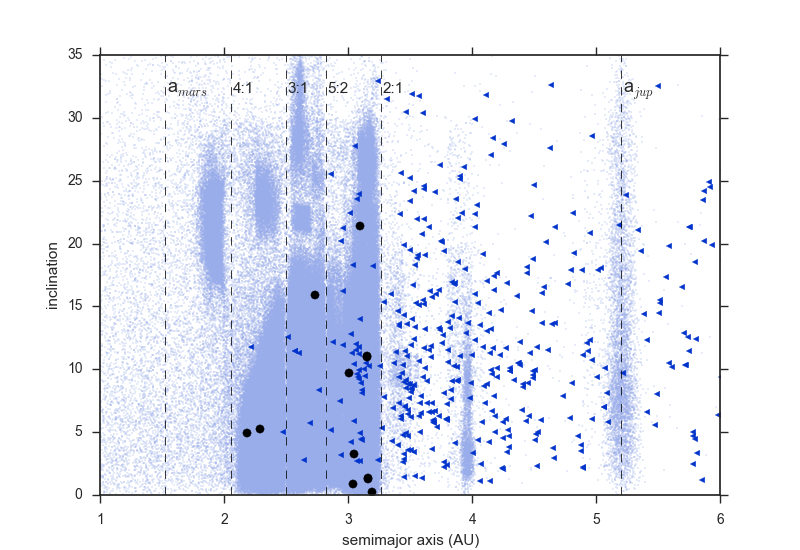
\includegraphics[height=9cm]{graphs/aa_comets_mba_all.png}
%    \caption{Inclination of all objects in the main asteroid belt from the AstDys catalogue as a function of semimajor axis.  Mean motion resonances between Mars and Jupiter as well as the planet's semimajor axis are marked in dashed lines, main belt objects are marked as light small dots, comets as arrows, and active asteroids as stars.}\label{fig:1}
%\end{figure}



\begin{figure}[!htb]
    \centering
    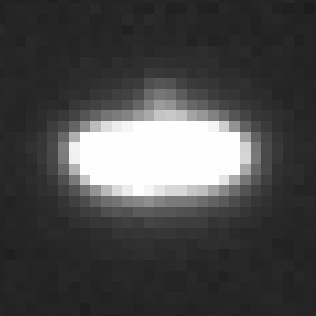
\includegraphics[height=4cm]{images/involved2_copy.png}
    \caption{An asteroid involved with a dim background object. }\label{fig:3}
\end{figure}


\end{document}



